\chapter*{Preface}
\addcontentsline{toc}{chapter}{Preface}
Theses at the Faculty of Mathematics and Physics of Charles University in Prague usually fit into one of three categories:
\begin{enumerate}
\item Theoretical thesis
\item Experimental thesis
\item Implementation thesis
\end{enumerate}
My thesis does not fit entirely into only one category and it does not try to. The project consists of several similarly important parts which are:
\begin{itemize}
\item Design of algorithms for generating a special binary matrix
\item Making the algorithms run fast on inputs that are usual for researchers
\item Implementation of the algorithms to provide a practical tool
\end{itemize}
One part would not make sense without others, but together, the thesis may become a very useful tool for scientists interested in matrices with forbidden patterns as the thesis provides them with a process of generating random pattern-avoiding matrices.

Implemented program is available here: \cite{program}.
\chapter*{Introduction}
\addcontentsline{toc}{chapter}{Introduction}
Throughout the thesis, we will be concerned with binary matrices and something called \emph{pattern}, which will also be a binary matrix.
\begin{defn}
We let $M\in\{0,1\}^{m\times n}$ denote a \emph{binary matrix} of size $m$~by~$n$. The \emph{height} of $M$, denoted by $m$, is the number of rows of $M$ and $n$ is its width (the number of columns).
\end{defn}
\begin{defn}
A \emph{line} of a matrix is one of its rows or columns and we denote by $L(M)$ the ordered set of all lines of $M$. Its order is given by the standard indexing of rows and columns, where the first index is zero and we put rows before columns. Example can be found in Figure~\ref{avoiding}.
\end{defn}
\begin{defn}
We say a binary matrix~$M$ \emph{contains} a binary matrix~$P$, which we call a pattern, as a submatrix, if there is a mapping~$f:L(P)\rightarrow L(M)$, such that
\begin{itemize}
\item $l\in L(P)$ is a row of $P$ if and only if $f(l)\in L(M)$ is a row of $M$
\item $\forall l,l'\in L(P):$ $l<l'\Rightarrow f(l)<f(l')$ (preserves the order)
\item $\forall l,l'\in L(P):$ if lines $l$ and $l'$ intersect and there is a one-entry at the intersection, then there is a one-entry at the intersection of $f(l)$ and $f(l')$.
\end{itemize}
Otherwise, it \emph{avoids} the pattern~$P$.
\end{defn}
\begin{figure}[h!]
\centering
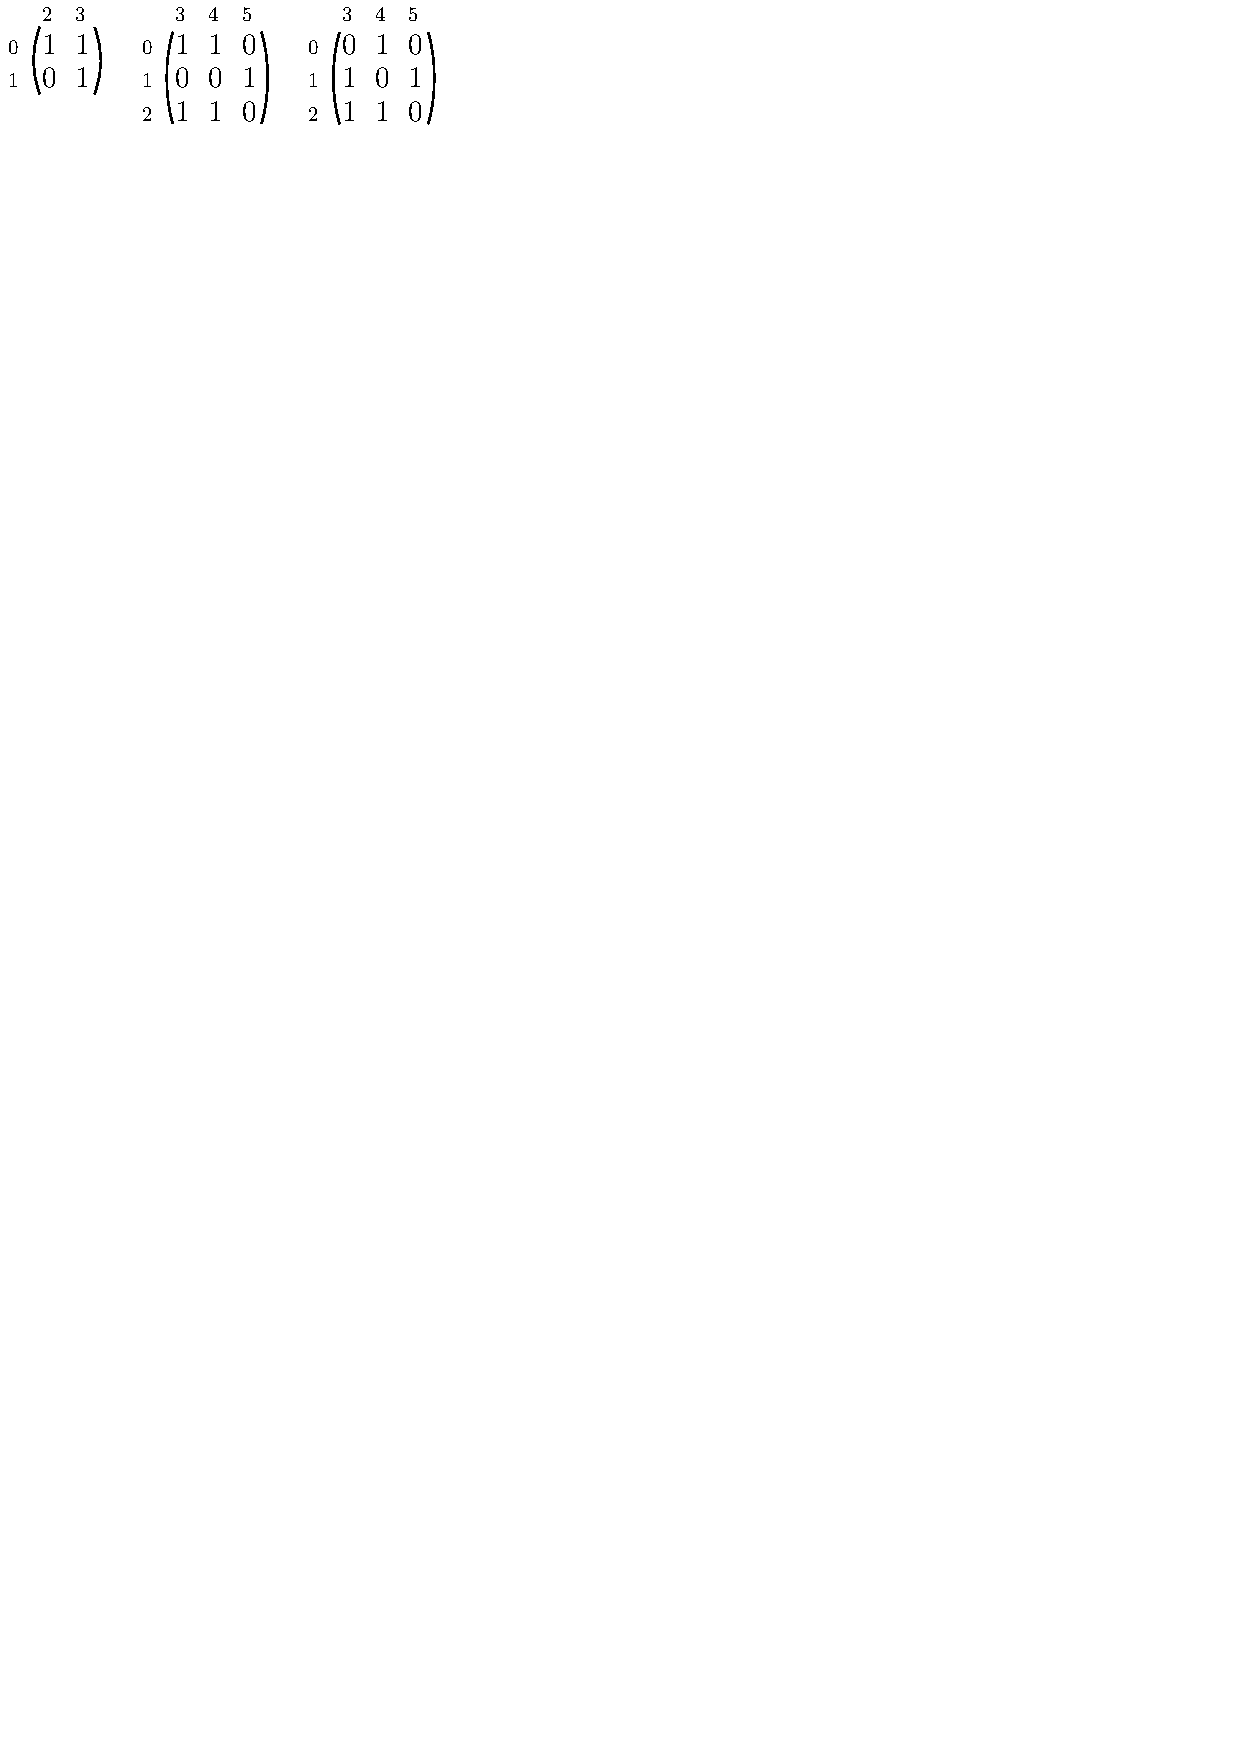
\includegraphics[width=100mm]{../img/avoiding.pdf}
\caption{Matrix~$M_1$ contains the pattern~$P$, because all the conditions are satisfied by mapping $\{(0,0),(1,2),(2,3),(3,4)\}$. On the other hand, matrix~$M_2$ avoids~$P$ as there is no such mapping.}
\label{avoiding}
\end{figure}

The interesting cases are square matrices of size $n$~by~$n$, where $n$ is big (going to infinity) and the size of a pattern (not necessarily square matrix) is small (constant). Even for a constant size forbidden pattern it is hard to determine the number of matrices of size $n$ that avoid it or to describe their properties. That is why it is useful to have a tool generating random matrices. Sometimes we consider matrices avoiding more than just one forbidden pattern, in which case we denote the set of all forbidden matrices by $\mathcal{P}$. When a matrix avoids $\mathcal{P}$, it avoids every $P\in\mathcal{P}$. 
\begin{ntn}
We denote by $\mathcal{M}_n(\mathcal{P})$ a set of all binary matrices of size $n$~by~$n$ avoiding $\mathcal{P}$ as submatrices.
\end{ntn}
\begin{ntn}
We always call $M$ the square binary matrix, for which we test the containing, and $P$ the pattern (if there is only one) that is being tested. Moreover, we denote by $h$ the height (the number of rows) of $P$ and by $w$ its width.
\end{ntn}
The area of pattern avoidance has been heavily studied for permutations and it also becomes more popular for their generalization -- binary matrices. In most of the areas in combinatorics, it is useful to explore properties of random objects and a lot of attention is directed towards random matrices when considering pattern avoidance. The goal of the thesis is, for given $n\in\mathbb{N}$ and set of forbidden patterns~$\mathcal{P}$, to generate a uniformly random $M\in\mathcal{M}_n(\mathcal{P})$.
\begin{figure}[h!]
\centering
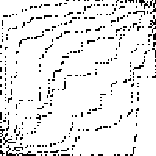
\includegraphics[width=60mm]{../img/walking-diag.pdf}
\caption{Example of a generated matrix avoiding $I_{10}$ (unit matrix). Black dots are one-entries and white are zero-entries. As you can see, matrices avoiding a pattern can have a nice structure.}
\label{avoiding}
\end{figure}
\subsection*{Generating random matrices}
\begin{ntn}
Let $A$ be a set and $a\in A$ be its element. By $a\in_R A$ we denote that $a$ is a uniformly random element of $A$.
\end{ntn}
One way to get $M\in_R\mathcal{M}_n(\mathcal{P})$ is to choose a matrix of required size completely at random, for such, test whether it avoids the pattern and simply repeat the process until we find one which does. However, in the most interesting cases, only a small fraction of all matrices avoid the pattern and the process takes too long, to be practically useful.

For generating random permutations avoiding a forbidden pattern, a different technique was introduced in \cite{MadrasLiu-mcmc}. It uses a randomized process called Markov chain Monte Carlo, which we will abbreviate by MCMC. It is an iterative process, which for a well chosen Markov chain (more in Chapter~\ref{chap:mcmc}) approximates a random object. The algorithm by Madras and Liu was developed for permutations (permutation matrices) and it cannot be used for general matrices. In Section~\ref{sect:mmcmc} we show how to adapt the algorithm, which will lead us to a MCMC algorithm that approximates $M\in_R\mathcal{M}_n(\mathcal{P})$. To produce a good approximation the process needs to do a lot of iterations. While the mixing time (the number of iterations required) of a MCMC process is unknown, in practice, the method does better than the trivial algorithm.
\subsection*{Testing avoidance}
In each step of our MCMC process, we need to test whether a matrix avoids a pattern. We will show a very fast algorithm that only works for a special class of binary matrices (explained in Chapter~\ref{chap:walking}) together with a slightly less efficient algorithm for a general pattern, which, again, comes as a generalization of an algorithm for permutations from the article by Madras and Liu and is described in Chapter~\ref{chap:general}.

In Chapter~\ref{chap:imp}, we improve both our algorithms and introduce a parallel version of MCMC process, which further increases the performance of matrix generating.

Some technical details are explained in Chapter~\ref{chap:tdoc} to make reading the code (\cite{program}) easier for the reader. The last chapter (Chapter~\ref{chap:udoc}) contains the user documentation.